\chapter{文獻探討}

\section{小標題}

\zhlipsum[1][name=trad]

測試圖片如圖 \ref{fig:figure_ref},測試論文引用 \cite{Ymc}。

\begin{figure}[h]
  \centerline{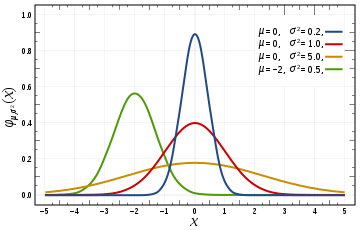
\includegraphics[width=0.5\columnwidth]{Images/gambar.png}}
  \caption{Gaussian distribution1}
  \label{fig:figure_ref}
\end{figure}

\subsection{小小標題}

方程式測試。方程式\ref{eq:index_eq},測試演算法。演算法\ref{alg:alg1}

\begin{equation}
  \label{eq:index_eq}
  (\hat{n})=\operatorname*{arg\,max}_{n\in \{1,\dots,M\}}(\mathbf{X}_{n})
\end{equation}
 
\begin{algorithm}
	\caption{test}
  \label{alg:alg1}
\end{algorithm}

\subsection{小小標題}

\zhlipsum[1][name=trad],表\ref{table:table1}


\begin{table}[h!]
  \begin{center}
    \caption{This is the example of table1}
    \label{table:table1}
    \begin{tabular}{|l|c|c|c|}
      \hline
      \textbf{Layer} & \textbf{Col1} & \textbf{Col2} \\ % <-- added & and content for each column
      \hline
      Row1 & content & content \\ % <--
      Row2 & a & b \\ % <--
      Row3 & c & d \\ % <--
      Row4 & e & f \\ % <--
      \hline
    \end{tabular}
  \end{center}
\end{table}
\subsubsection{小小小標題}